
%FORME LAGRANGIENNE DE LA MECANIQUE QUANTIQUE

 \chapter{Introduction}
\section{Les Postulats de la mécanique Quantique}

Les postulats de la mécanique quantique sont de deux
natures essentiellement différentes :
\subsection{Les postulats généraux}
Ce sont les postulats fondamentaux, qui
sont communs à tous les exposés de la mécanique quantique :

\subsubsection{Principe de superposition}
Les états d'un système
physique sont linéairement superposables : si | $\psi_1$ > et | $\psi_2$ > sont
deux états du système, $\lambda_1$ | $\psi_1$ > $+ \lambda_2$ | $\psi_2$ >
représente également un état du système ($\lambda_1, \lambda_2$ complexes).

Rappelons en fait que les états physiques sont représentés
par des vecteurs d'un espace de Hilbert. Les grandeurs physiques sont
alors représentées par des opérateurs hermitiques à spectre complet
(observables) de cet espace. Les | U$_\mt{n}$ > étant les vecteurs propres
(de valeur propre a$_\mt{n}$) de l'observable A :
\begin{center}
A | U$_\mt{n}$ > $=$ a$_\mt{n}$ | U$_\mt{n}$ >
\end{center}
il existe entre les | U$_\mt{n}$ > les relations d'orthogonalité et de
fermeture :
\begin{center}
< U$_\mt{n}$ | U$_\mt{n'}$ > $=$ $\delta_\mt{nn'}$

$\sum$ | U$_\mt{n}$ > < U$_\mt{n}$ | $=$ 1
\end{center}

% - 2
\subsubsection{Caractère probabiliste}
Le système physique étant dans
l'état | $\psi$ >, le résultat de la mesure d'une grandeur physique représentée
par l'observable A ne peut être que l'une des valeurs propres
a$_\mt{n}$ de À et la probabilité pour que ce résultat soit a$_\mt{n}$ est
| < U$_\mt{n}$ | $\psi$ > |$^2$, carré du module de l'{\it amplitude de probabilité}
< U$_\mt{n}$ | $\psi$ >.
\subsection{Les postulats de quantification}
Pour trouver les observables associées aux grandeurs physiques,
les relations de commutation entre
ces observables et l'équation d'évolution des vecteurs d'état et des
observables, on fait appel aux postulats de quantification. Ceux-ci
peuvent prendre une {\it forme différente} d'un exrosé à l'autre de la
mécanique quantique. On leur impose toutefois une condition : si on
quantifie un systère classique, on doit retrouver les propriétés classiques
à la limite où l'on fait tendre H vers zéro. Les postulats de
quantification doivent ainsi traduire une certaine analogie entre les
mécaniques classique et quantique .

Avant de passer en revue différents formalismes possibles de
quantification, revoyons rapidement les formes que peut prendre le
mécanique classique.
\section{Les différentes formes de la mécanique classique}

\subsection{La forme Mewtonienne}
Elle est basée sur l'équation fondamentale de la dynamique, $\vec{F}$ $=$ m$\vec{\gamma}$

\subsection{La forme Lagrangienne}
On définit pour chaque système un lagrangien,
fonction des ''coordonnées généralisées'' q et de leur dérivée par rapport
au temps. Dans le cas d'une particule définie par ces coordonnées q = x,
dans un potentiel V(x), le lagrangien s'écrit

\begin{center}
$\mt{L}$ $[$ x(t), $\pt{x}$(t) $]$ $= \frac{1}{2}$ m $\pt{x}^2$ $-$ V(x) 
\end{center}
% - 3
A partir du lagrangien, on construit l'action
\[
\mt{S} = \int_\mt{t'}^\mt{t''} \mt{L} [ \mt{x(t)}, \pt{\mt{x}}\mt{(t)} ] \mt{dt}
\]
Parmi toutes les trajectoires x(t) possibles entre un point
x' à l'instant t' et un point x'' à l'instant t'', la traiectoire {\it réellement} suivie sera celle qui rend l'action S {\it stationnaire}. C'est le principe variationnel de Hamilton ou de moindre action. On déduit de ce
principe les équations de Lagrange, système d'équations différentielles
du second ordre, et on montre l'équivalence avec le principre fondamental
de la dynamique newtonienne.

\begin{center} \begin{tikzpicture}
\draw [->] (0,0) --++ (5,0) node [below] {t};
\draw [->] (0,0) --++ (0,4) node [left] {x};
\node at (0,0) [left]{O};
\draw [densely dashed] (0,3) node [left] {x'} --++ (1,0);
\draw [densely dashed] (1,0) node [below] {t'} --++ (0,3);
\node at (1,3) [above]{M'};
\draw [densely dashed] (0,1) node [left] {x''} --++ (4,0);
\draw [densely dashed] (4,0) node [below] {t''} --++ (0,1);
\node at (4,1) [right]{M''};
\draw [line width=1.5pt] (1,3) .. controls (1.9,3) and (3.9,1.9) .. (4,1);
\end{tikzpicture} \end{center}

\subsection{La forme Hamiltonienne}
L'évolution du système est décrite à l'aide
de 1a fonction de Hamilton des coordonnées q et des ''moments conjugués''
p $=$ $\frac{\partial \mt{L}}{\partial \pt{q}}$, H(p, q).

La trajectoire se détermine à l'aide des équations canoniques

\[
\frac{\mt{dq}_\mt{i}}{\mt{dt}} = \frac{\partial \mt{H}}{\partial \mt{p}_\mt{i}}
\ \ \ ;\ \ \ \ 
\frac{\mt{dp}_\mt{i}}{\mt{dt}} = \frac{\partial \mt{H}}{\partial \mt{q}_\mt{i}}
\]

qui sont du premier degré,
C'est en général à rartir de cette dernière forme que l'on bâti
la mécanique quantique.
% - 4
\section{Forme habituelle des règles de quantification}

On part de la forme hamiltonienne de la mécanique classique
et on postule (principe de correspondance) la relation entre commutateurs
et crochets de Poisson :

\begin{center}
$[$ A, B $]$ $=$ i$\hbar$ \{ A, B \}
\end{center}

Rappelons la définition des crochets de poisson :
\[
\{\mt{ A, B }\} = \sum_\mt{i}
(\frac{\partial \mt{A}}{\partial \mt{q}_\mt{i}}\frac{\partial \mt{B}}{\partial \mt{p}_\mt{i}}
- \frac{\partial \mt{A}}{\partial \mt{p}_\mt{i}}\frac{\partial \mt{B}}{\partial \mt{q}_\mt{i}}).
\]
On en déduit notamment les commutateurs fondamentaux $[$ q, p $]$ $=$ i$\hbar$,
l'équation de Schrôdinger, etc.

Ce formalisme hamiltonien a l'avantage de se prêter aisément
aux calculs. Cependant, la forme lagrangienne de la mécanique classique
est plus fondamentale que la forme hamiltonienne : elle découle en effet
d'un principe variationnel et peut ainsi se généraliser à tout système
physique régi par un tel principe. Enfin, elle fait jouer au temps un
rôle plus symétrique que la forme hamiltonienne, où le temps est très
particularisé. Elle pourra donc prendre plus facilement une forme invariente relativiste.
Il est donc intéressant de donner une règle de quantification de la mécanique lagrangienne.
Pour bien comprendre le sens
physique de cette règle, analysons d'abord le passage entre l'optique
géométrique et l'optique ondulatoire :
\section{Passage de l'optique géométrique à l'optique ondulatoire}
L'optique géométrique est régie par le Principe de Fermat :

\begin{center} \begin{tikzpicture}
\draw [->] (0,0) --++ (5,0) node [below] {y};
\draw [->] (0,0) --++ (0,4) node [left] {x};
\node at (0,0) [left]{O};
\draw [densely dashed] (0,3) node [left] {x'} --++ (1,0);
\draw [densely dashed] (1,0) node [below] {y'} --++ (0,3);
\node at (1,3) [above]{M'};
\draw [densely dashed] (0,1) node [left] {x''} --++ (4,0);
\draw [densely dashed] (4,0) node [below] {y''} --++ (0,1);
\node at (4,1) [right]{M''};
\draw [line width=1.5pt] (1,3) .. controls (1.9,3) and (3.9,1.9) .. (4,1);
\end{tikzpicture} \end{center}
 
Le chemin suivi par la lumière de M' à M'' correspond au
temps de parcours {\it minimum} ; de façon plus précise, il correspond à un
temps stationnaire, c'est-à-dire qu'une variation au premier ordre du
chemin autour du chemin suivi entraîne une variation du temps au second
ordre. Notons que les chemins en question ici sont des chemins d'espace
ordinaire (décrits en xy) et non des chemins d'espace temps (décrits en
xt) comme dans le principe de Hamilton.

Un exemple du principe de Fermat est fourni par les lois de
la réflexion, le chemin M'PM'' suivi par la lumière entre M' et M'' étant
extremum parmi tous les chemins M'QM'' possibles.

\begin{center} 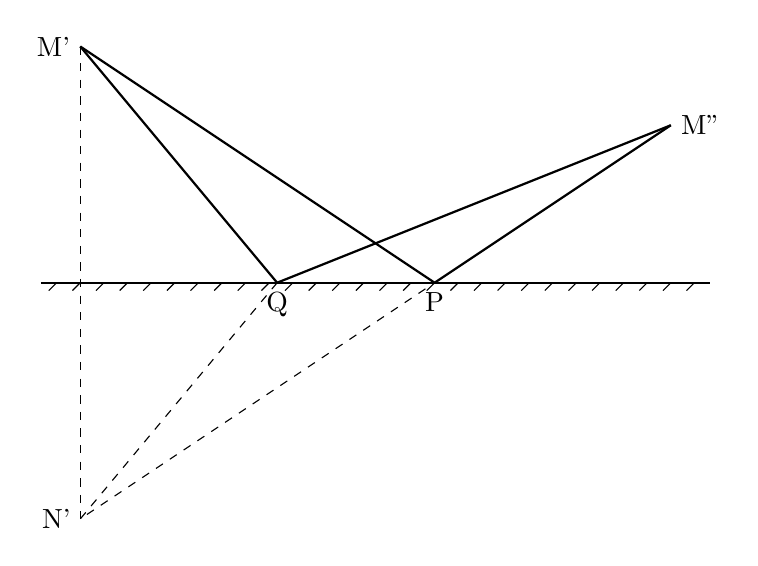
\begin{tikzpicture}
%miroir
\draw[thick] (0,0)--(8.5,0);
\foreach \z in {0.2,0.5, ...,8.5}
{\draw (\z,0)--++(-0.1,-0.1);}
%rayons
\draw [thick] (0.5,3) node [left]{M'} -- (5,0) node [below]{P} -- (8,2) node [right]{M''};
\draw [thick] (0.5,3) -- (3,0) node [below]{Q} -- (8,2);
%symétrique
\draw [dashed] (0.5,3) -- (0.5,-3) node [left]{N'};
%virtuels
\draw [dashed] (3,0) -- (0.5,-3) -- (5,0);
\end{tikzpicture} \end{center}

Une question importante se pose alors : comment le rayon
lumineux trouve-t-il le chemin de temps stationnaire ? La réponse vient
du caractère ondulatoire de la lumière qui lui permet de “sentir” tous
les chemins possibles.

L'{\it optique ondulatoire} peut se résumer dans le {\bf Principe
d'Huyghens} : Soit $\phi$ (M'', M') l'amplitude de l'onde lumineuse issue de
M' et arrivant en M'' (l'intensité de l'onde est alors | $\phi$ (M'', M') |$^2$).
Le principe d'Huyghens dit que $\phi$ (M'', M') est une somme de contributions,
\begin{center} 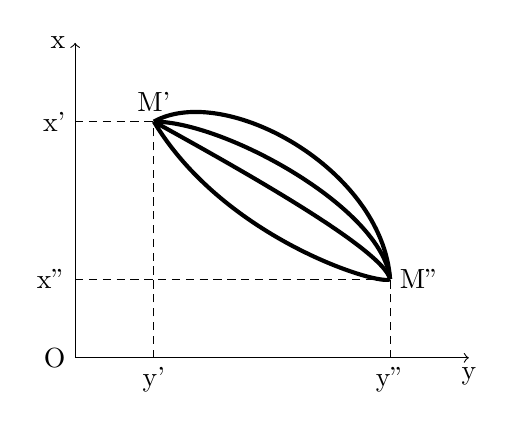
\begin{tikzpicture}
% axes
\draw [->] (0,0) --++ (5,0) node [below] {y};
\draw [->] (0,0) --++ (0,4) node [left] {x};
\node at (0,0) [left]{O};
% coordonnées et points
\draw [densely dashed] (0,3) node [left] {x'} --++ (1,0);
\draw [densely dashed] (1,0) node [below] {y'} --++ (0,3);
\node at (1,3) [above]{M'};
\draw [densely dashed] (0,1) node [left] {x''} --++ (4,0);
\draw [densely dashed] (4,0) node [below] {y''} --++ (0,1);
\node at (4,1) [right]{M''};
% Chemins
\draw [line width=1.5pt] (1,3) .. controls (1.9,3) and (3.9,1.9) .. (4,1);
\draw [line width=1.5pt] (1,3) .. controls (1.9,3.5) and (3.9,2.4) .. (4,1);
\draw [line width=1.5pt] (1,3) .. controls (1.9,2.5) and (3.9,1.4) .. (4,1);
\draw [line width=1.5pt] (1,3) .. controls (1.9,1.5) and (3.9,0.9) .. (4,1);
\end{tikzpicture} \end{center}
%-6
une pour chaque chemin partant de M' et arrivant en M''. La contribution
de chaque chemin est un nombre complexe dont le module peut être considéré
en première approximation comme constant et dont la phase est
2i$\pi \frac{\mt{t}_\mt{c}}{\mt{T}}$, t$_\mt{c}$ étant le temps mis pour parcourir le chemin en question
et T la période de vibration. Par exemple, dans le cas de la réflexion, le chemin M'QM'' contribue à
$\phi$ (M'', M') par le terme exp(2i$\pi \frac{\mt{M'Q + QM''}}{\mt{cT}}$). (cT $=$ $\lambda$ : longueur d'onde).

Dans le cas limite où toutes les dimensions sont grandes devant
la longueur d'onde $\lambda$ (mathématiquement T $\to$ O ou encore $\lambda$ = cT $\to$ 0), d'un
chemin à l'autre la phase varie très vite, Les seuls chemins dont les
contributions ne se détruisent pas par interférence, sont ceux pour lesquels la phase est stationnaire
(c'est-à-dire ceux pour lesquels une variation du chemin au premier ordre entraîne une variation de phase
au deuxième ordre). Tout se passe comme si on pouvait ignorer tous les chemins autres que les chemins de
phase stationnaire, c'est-à-dire de temps
stationnaire. Physiquement, cela veut dire que rien n'est changé à l'amplitude  $\phi$ (M'', M')
si on internose
un écran qui cache les chemins non
stationnaires, à condition que le diaphragme ait des {\it dimensions grandes}
devant $\lambda$. Tout se passe donc alors comme si la lumière suivait les chemins du {\it principe de Fermat}.

Le Principe de Huyghens contient donc le principe de Fermat à
la limite où $\lambda$ $\to$ O.

Dans le cas où $\lambda$ ne peut être considéré comme négliseable,
l'optique géométrique ne {\it s'applique plus} et les phénomènes doivent être
décrits à l'aide du principe d'Huyghens : c'est le cas des expériences
de diffraction.

Le passage de la mécanique classique à la forme laprangienne
de la mécanique quantique repose sur la même idée de base.
% - 7
\section{Idée de base de la formulation lagrangienne de la mécanique quantique}
La mécanique classique est basée sur le {\bf principe de Hamilton} :
le chemin x(t) suivi par la particule correspond à l'action stationnaire
(remarquons que nous raisonnons à nouveau dans l'espace temps (x, t) et
non plus dans l'espace ordinaire (x y)).

\begin{center} 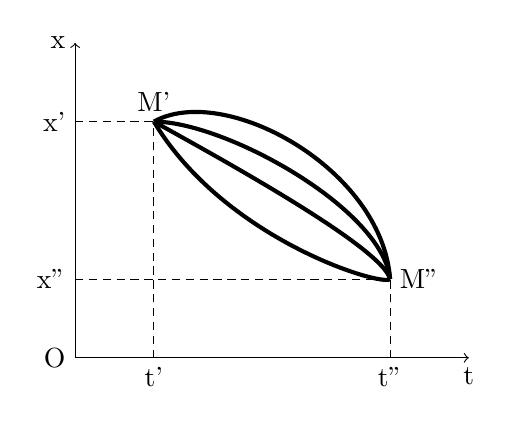
\begin{tikzpicture}
% axes
\draw [->] (0,0) --++ (5,0) node [below] {t};
\draw [->] (0,0) --++ (0,4) node [left] {x};
\node at (0,0) [left]{O};
% coordonnées et points
\draw [densely dashed] (0,3) node [left] {x'} --++ (1,0);
\draw [densely dashed] (1,0) node [below] {t'} --++ (0,3);
\node at (1,3) [above]{M'};
\draw [densely dashed] (0,1) node [left] {x''} --++ (4,0);
\draw [densely dashed] (4,0) node [below] {t''} --++ (0,1);
\node at (4,1) [right]{M''};
% Chemins
\draw [line width=1.5pt] (1,3) .. controls (1.9,3) and (3.9,1.9) .. (4,1);
\draw [line width=1.5pt] (1,3) .. controls (1.9,3.5) and (3.9,2.4) .. (4,1);
\draw [line width=1.5pt] (1,3) .. controls (1.9,2.5) and (3.9,1.4) .. (4,1);
\draw [line width=1.5pt] (1,3) .. controls (1.9,1.5) and (3.9,0.9) .. (4,1);
\end{tikzpicture} \end{center}
Comment la particule trouve-t-elle le chemin d'action minimum ?
La réponse est fournie par la théorie quantique : elle “sent” les autres
chemins grâce à son aspect ondulatoire,

Appelons < x''t'' | x't' > l'{\it amplitude de probabilité} pour que la
particule, soit en x'' à l'instant t'' après avoir été en x' à l'instant t'.
< x''t'' | x't' > est une {\it somme} de contributions, une pour chaque chemin
d'espace temps partant de x't' et arrivant en x''t'', La contribution d'un
chemin donné s'écrit : N exp(2i$\pi \frac{\mt{S}}{\mt{h}}$). N est un coefficient de normalisation
indépendant du chemin; S est l'action classique $\int_\mt{t'}^\mt{t''}$ L (x,$\pt{x}$) dt calculée
le long du chemin considéré, h la constante de Planck, qui a bien les
dimensions d'une action (S/h est donc sans dimensions). C'est le {\bf principe
de quantification de Feynman}.

A la limite où $\hbar$ $\to$ 0, les seuls chemins qui contribuent à
< x''t'' | x't' > sans se détruire par interférence correspondent à une
phase stationnaire, donc à une action stationnaire.

% -8
Le Principe de Feynman contient donc le principe de Hamilton
à la limite où $\hbar$ $\to$ 0.

Il existe donc une analogie précise entre l'optique géométrique
et la mécanique classique d'une part, l'optique ondulatoire et la mécanique quantique d'autre part,
l'action remplaçant le temps et la constante
de Planck la période de l'onde lunineuse,

On peut donc dire qu'une expérience de mécanique quantique est
une expérience de diffraction dans l'espace-temps; toutes les propriétés
ondulatoires de la matière apparaissent clairement dans cette formulation
de la mécanique quantique, dont il reste encore à montrer qu'elle est
bien équivalente aux autres.

Résumons, pour terminer, les avantages de ce nouveau point de vue :

1°) Il donne un sens physique plus clair à la correspondance
entre la mécanique classique et la mécanique quantique.

2°) On raisonne dans l'espace-temps, ce qui permet un passage
à la relativité très aisé : il suffit de remplacer dt par d$\tau$, $\tau$ étant le
temps propre de la particule, et prendre pour Lagrangien L une fonction
scalaire d'espace-temps. L'action S = $\int$ L d$\tau$ est alors un scalaire et la
théorie acquiert l'invariance relativiste.

Dans la formulation hamiltonienne au contraire, le temps
est très privilégié et la covariance relativiste des équations n'est pas
apparente.

3°) Le point de vue est plus global : au lieu de considérer des
amplitudes de probabilité pour un état à un instant donné, on associe une
amplitude de probabilité à une {\it histoire entière}, ou chemin, du système.
Ce point de vue se révèle souvent plus fructueux et plus intéressant.

4°) Ce procédé est applicable à des systèmes autres que mécaniques,
à la seule condition que leurs équations classiques découlent d'un
{\it principe variationnel} : c'est le cas du champ électromagnétique dont les
% - 9
équations de Maxwell peuvent se déduire d'un Lagrangien et d'un principe
d'action stationnaire.

La quantification se fait alors en associant à chaque histoire
du champ une amplitude de probabilité proportionnelle à exp(2i$\pi \frac{\mt{S}}{\mt{h}}$).

On voit ainsi l'importance de ce formalisme en théorie quantique
des champs.
